\documentclass[conference]{IEEEtran}
\IEEEoverridecommandlockouts
\usepackage{cite}
\usepackage{amsmath,amssymb,amsfonts}
\usepackage{algorithmic}
\usepackage{graphicx}
\usepackage{textcomp}
\usepackage{xcolor}
\usepackage{float}

\def\BibTeX{{\rm B\kern-.05em{\sc i\kern-.025em b}\kern-.08em
    T\kern-.1667em\lower.7ex\hbox{E}\kern-.125emX}}
\begin{document}

\title{Comparison of NumPy vs Python Implementaion of Strassen's Algorithm for Embedded Devices 
}

\author{\IEEEauthorblockN{Vishakha Dixit}
\IEEEauthorblockA{\textit{ECE Department - 801265288} \\
\textit{University of North Carolina at Charlotte}\\
    Charlotte, NC \\
    vdixit2@uncc.edu}
}

\maketitle

\begin{abstract}
    This document explores simple experiments that contrast two Python Implementaion of matrix-matrix multiply. It also compares 
    their performance metrics to help understand which approach is most suitable for small Embedded Devices like Raspberry Pi.

\begin{IEEEkeywords}
    NumPy, Strassen, Embedded, RaspberryPi
\end{IEEEkeywords}
\end{abstract}

\section{Introduction}
    Python first emerged in the 1990s and has steadily gained popularity among software developers since then. Initially, 
    Python became popular amongst embedded developers as a scripting language to test electronic devices. Slowly it has been 
    moving further down the development stack. The Python programming language provides a rich set of high-level data structures: 
    lists for enumerating a collection of objects, dictionaries to build hash tables, etc. However, these structures are not ideally 
    suited to high-performance numerical computation. The NumPy package in python provides better ways of handling data for Mathematical 
    Operations. The questions here is, does NumPy also enable efficient use of resources for Embedded Devices such as Raspberry Pi, 
    where we have limited RAM, Flash memory, and CPU power consumption restraints? 

\section{Background}

    The Raspberry Pi 3 module is used for the purpose of this research. It is a low-cost single board computer that enables people 
    of all ages to explore computing, and to learn about how to program in languages such as Python. Raspberry pi can also be used 
    for development of complex applications such as Motion detection using webcam. Motion detection requires processing of every 
    frame captured by the Raspberry pi camera module. Processing of frames can be CPU and Memory intensive, also power consumption 
    for such application can be very high. This experiment explores different implementations using python and NumPy package. 

\section{Description of Experimental Infrastructure}
    Image processing involves extraction, filtering, enhancement etc. of images using mathematical operations. Every digital image has 
    a corresponding matrix of color and color intensities. Various mathematical operations are performed on these matrices for enhancing 
    the corresponding image.

    This experiment uses Python programming language and two Python implementations of matrix-matrix multiply. Both these methods solve 
    same problem of matrix multiplication. This experiment compares Python Implementation of Strassen\textquotesingle s Algorithm with NumPy 
    library\textquotesingle s matrix multiplication function. The results are measured by comparing Execution time, CPU Utilization, 
    and RAM Utilization. 

    The execution time parameter is being measured to quantify for how long the system needs to be in high power state to process 
    the data. CPU Utilization measures how efficiently the process utilizes available CPU. Memory Utilization measures how much RAM 
    is used by the process.
    
    Python\textquotesingle s psutil library is used to measure CPU and RAM Utilization, whereas time library is used to compute the execution 
    time of the process.


\subsection{Scope}
    This experiment uses following three different matrix dimensions:
    \begin{itemize}
        \item 64x64: represents low resolution image
        \item 256x256: represents an image closer to 360p resolution
        \item 1024x1024: represents high resolution image closer to 1080p
    \end{itemize}

    The dimensions taken here are in powers of 4 to create square matrix because Strassen\textquotesingle s Algorithm uses recursive approach for matrix multiplication 
    where in each recursive step it divides the matrix into 4 sub matrices of dimensions n/2 x n/2.

\section{Results And Analysis}
    Following results were obtained after running both the Algorithms for all three dimensions mentioned in the Scope: 
    \begin{table} [H]
        \centering
        \begin{tabular}{ | c | c | c | c | }
        \hline
        \textbf{Algorithm} & \textbf{64x64} & \textbf{256x256} & \textbf{1024x1024} \\ [1.0 ex]
        \hline 
        Strassen\textquotesingle s & 22884352 & 26177536 & 63369216 \\ [1.0 ex]
        \hline
        NumPy\textquotesingle s Matmul & 22794240 & 24301568 & 48500736 \\ [1.0 ex]
        \hline 
        \end{tabular}\\ [1.0 ex]
        \caption{Memory Usage in Bytes}
        \label {table:1}
    \end{table}

    \begin{table} [H]
        \centering
        \begin{tabular}{ | c | c | c | c | }
        \hline
        \textbf{Algorithm} & \textbf{64x64} & \textbf{256x256} & \textbf{1024x1024} \\ [1.0 ex]
        \hline 
        Strassen\textquotesingle s & 3261.342 & 155599.74 & timed-out \\ [1.0 ex]
        \hline
        NumPy\textquotesingle s Matmul & 5.797 & 1794.550 & 222168.144 \\ [1.0 ex]
        \hline 
        \end{tabular}\\ [1.0 ex]
        \caption{Execution time in ms}
        \label {table:2}
    \end{table}

    \begin{figure}[htbp]
    \centerline{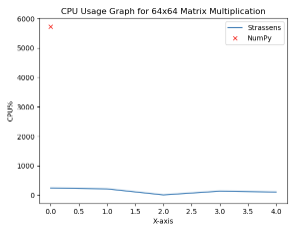
\includegraphics{CPU_Usage_64x64.png}}
    \label{fig1}
    \end{figure}

    \begin{figure}[htbp]
    \centerline{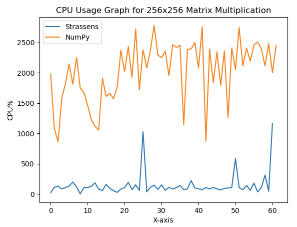
\includegraphics{CPU_Usage_256x256.png}}
    \label{fig2}
    \end{figure}

    \begin{figure}[htbp]
    \centerline{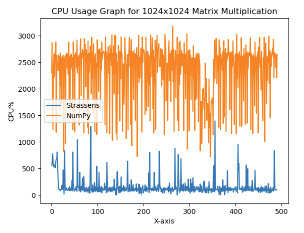
\includegraphics{CPU_Usage_1024x1024.png}}
    \label{fig2}
    \end{figure}
    
    
    Strassen\textquotesingle s Algorithm got progressively slower with increasing size of matrix. For 
    matrix of size 1024x1024, Strassen\textquotesingle s Algorithm couldn\textquotesingle t complete it\textquotesingle s execution
    and timed out after running for 10 minutes. 
    
    For NumPy implementation Cpu runs at full computational power but for less amount of time. Stranssen\textquotesingle s algorithm uses more memory 
    and is efficient while using the CPU.

\section{Conclusion}
    Numpy utilizes CPU resources more efficiently, hence the execution time required by NumPy is very low compared
    to Strassen\textquotesingle s Algorithm. Therefore, the devices can be kept in low power sleep mode for longer 
    period of time. Also, memory utilization in NumPy is less compared to regular python implementaion. Hence
    it is worth to use NumPy in an Embedded device, even though it might consume more Flash memory.

\begin{thebibliography}{00}
\bibitem{b1}\textbf{[NumPy]} Stefan van der Walt; S. Chris Colbert; Gael Varoquaux.
    The NumPy Array: A Structure for Efficient Numerical Computation, Computing in Science and Engineering,
    Volume: 13, Issue: 2, March-April 2011, doi:10.1109/MCSE.2011.37.
\bibitem{b2} \textbf{[IPython]} Fernando Perez, Brian E. Granger.
    IPython: A System for Interactive Scientific
    Computing, Computing in Science and Engineering,
    vol. 9, no. 3, pp. 21-29, May/June
    2007, doi:10.1109/MCSE.2007.53.
\end{thebibliography}

\end{document}
